\documentclass{article}

\usepackage{../template}

\usepackage{cleveref}
\usetikzlibrary{knots}

%\usepackage{asymptote}
\usepackage{asypictureB}

\usepackage{pgfplots}

\usepackage[strict]{changepage}

\usepackage{subfig}
% \usepackage{caption}
% \usepackage{subcaption}
%
% \DeclareCaptionFormat{subfig}{\figurename~#1#2#3}
% \DeclareCaptionSubType*{figure}
% \captionsetup[subfigure]{format=subfig,labelsep=colon,labelformat=simple}

\title{05: Wielomian Jonesa\\ węzłów alternujących}
\author{Weronika Jakimowicz}
\date{27.03.2024}

\declaretheorem[
   name=Fakt,
   numbered=no,
   style=uwagi-lematy
]{fuck}

\declaretheorem[
   name=Twierdzenie,
   numbered=no,
   style=twierdzonka
]{thm}

\renewcommand{\contentsname}{Spis sznurków}
 
\renewenvironment{proof}{{\bfseries\color{orange} Dowód}$ $\newline}{
  \begin{flushright}
\includegraphics[width=30pt]{Donald_Duck.png}\end{flushright}$ $\newline
}

\setcounter{secnumdepth}{0}


\begin{document}
\maketitle
\thispagestyle{empty}

\def\dupa{\textwidth - 4cm}
\begin{tikzpicture}[overlay, remember picture]
  \foreach \i in {0,..., 10} {
    \pgfmathparse{Mod(\i,2)==0?1:0)}
    \ifnum\pgfmathresult>0 
      \node at (4-1*\i,4.7) {
\includegraphics[width=1cm]{kaczusia.png}};
    \else 
      \node at (4-1*\i, 4.3) {
\includegraphics[width=1cm]{kaczusia.png}};
    \fi
  }
  \foreach \i in {0,..., 10} {%\node at (\dupa + \i*1cm, 4.5) {
\includegraphics[width=1cm]{kaczusia.png}};
    \pgfmathparse{Mod(\i,2)==0?1:0)}
    \ifnum\pgfmathresult>0 
      \node at (\dupa+\i*1cm,4.7) {
\includegraphics[width=1cm]{kaczusia.png}};
    \else 
      \node at (\dupa+\i*1cm, 4.3) {
\includegraphics[width=1cm]{kaczusia.png}};
    \fi
  }
\end{tikzpicture}


\tableofcontents\setcounter{page}{0}
\newpage 
\pagestyle{plain}

\subsection{Definicja węzła i linku alternującego}

Mówimy, że diagram regularny $D$ węzła $K$ jest alternujący, jeśli poruszając dowolny punkt $P\in D$ wzdłuż $D$, ciągle w jedną stronę, będziemy na zmianę pokonywać skrzyżowania górą i dołem.

\begin{deff}[węzeł alternujący]
  Węzeł $K$ jest alternujący, jeśli posiada przynajmniej jeden diagram alternujący.
\end{deff}

Najprostszy (o najmniejszej liczbie skrzyżowań) węzeł niealternujący to np. $8_{19}$ (ale też $8_{20}$ i $8_{21}$), który widać na \cref{diagram 8 19}. Do pokazania, że naprawdę nie kłamię jeśli chodzi o jego niealternującą naturę, wrócimy przy okazji powierzchni Seiferta i \emph{sygnatury węzła}.
\begin{figure}[h]\centering
  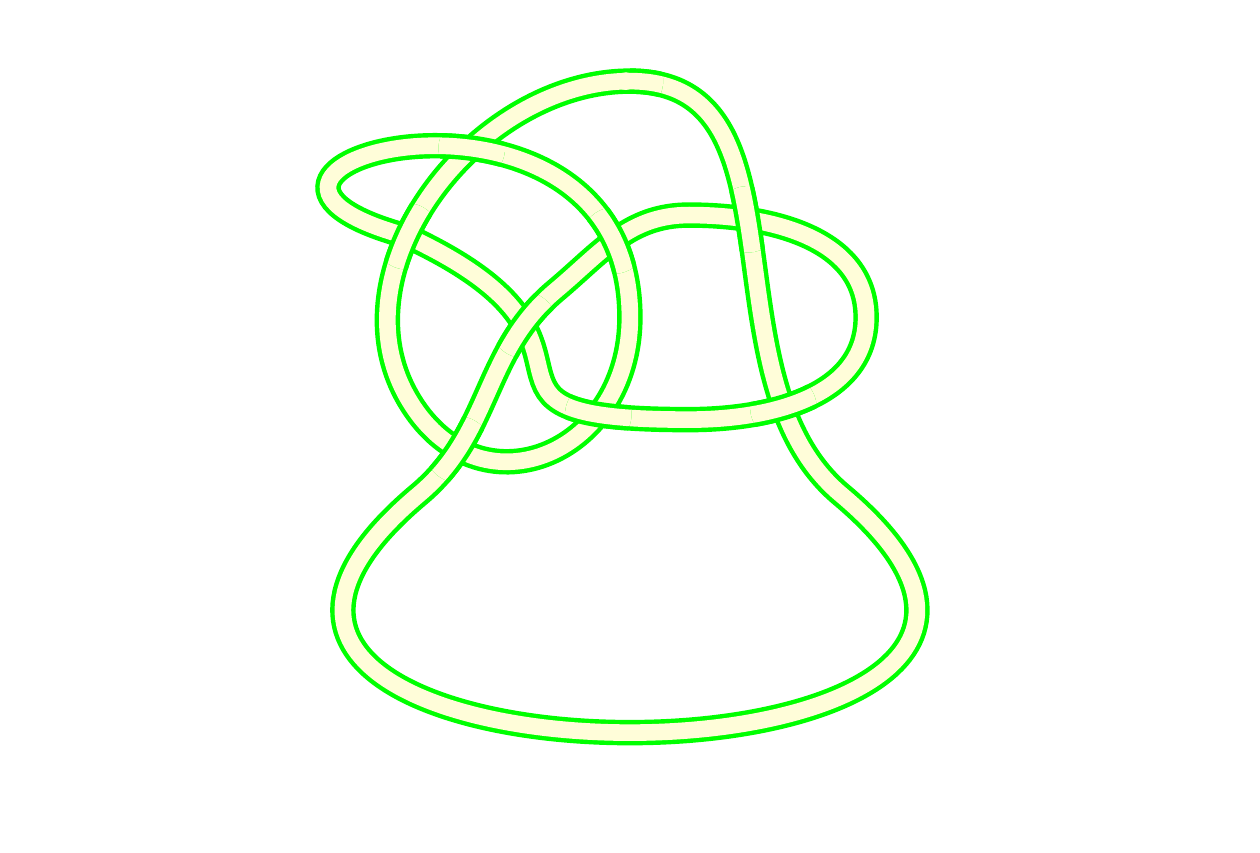
\begin{tikzpicture}
    \coordinate (a0) at (0,0);
    \coordinate (a1) at (90:3);
    \coordinate (a2) at (-40:3.5);
    \coordinate (a3) at (220:3.5);
    \coordinate (a4) at (160:1);
    \coordinate (a5) at (60:1.5);
    \coordinate (a6) at (0:3);
    \coordinate (a7) at (-60:1.5);
    \coordinate (a8) at (160:3);
    \coordinate (a9) at (200:3);

    %\foreach \i in {0,...,9} \fill (a\i) circle (3pt);
      
    \begin{knot}[
      clip width=2,
%      draft mode=crossings,
      consider self intersections,
      ignore endpoint intersections=false,
      flip crossing=2,
      flip crossing=6,
      flip crossing=8,
      line join=round,
      background color=white,
        only when rendering/.style={
        draw=green,
        ultra thick,
        double=yellow!15,
        double distance=6pt,
        %line cap=round,
      }
      ]
        \strand[thick] 
        (a1) to[out=0, in=140]
        (a2) to [out= -40, in=-140, looseness=3]
        (a3) to [out=40, in=-140]
        (a4) to [out=40, in=180]
        (a5) to [out=0, in=90]
        (a6) to [out=-90, in=0]
        (a7) to [out=180, in=-25, looseness=2]
        (a8) to [out=165, in=90, looseness=3]
        (a0) to [out=-90, in=-60, looseness=1.5]
        (a9) to [out=120, in=180]
        (a1);
    \end{knot}
    \fill[yellow!15] (91:3) circle (3.2pt);
  \end{tikzpicture}
  \caption{\label{diagram 8 19}Przykładowy diagram węzła $8_{19}$.}
\end{figure}

\begin{fuck}[alternująca suma spójna]
  Jeśli $K_1$ i $K_2$ są węzłami alternującymi o alternujących diagramach mających odpowiednio $n_1$ i $n_2$ skrzyżowań, to ich suma spójna $K_1\#K_2$ ma diagram alternujący o dokładnie $(n_1+n_2)$ skrzyżowaniach.
\end{fuck}

\begin{proof}
  Wiemy, że "na zewnątrz" węzła $K_1$ istnieje segment, pod którym przechodzi dokładnie jeden inny segment. Tak samo w przypadku diagramu $K_2$. Mamy dwie opcje, jak widać na \cref{fakt 1 dowodzik}.
  \begin{figure}[h]\centering
    \begin{tikzpicture}
      \begin{scope}[shift={(0, -7)}]
      \draw (-.2, 1.1)--(-.2, 1.7);
      \fill[white] (-.2, 1.4) circle (4pt);
      \draw[very thick] (2.5, -1.5)--(2.5, 1);
      \fill[white](2.5, -1) circle (4pt);
      \draw[very thick, blue] (2, -1)--(3, -1);
      \draw[very thick, red] (2, -2)--(3, -2);
      \fill[white] (2.5, -2) circle (4pt);
      \draw[very thick] (2.5, -4)--(2.5, -1.5);
      \draw[very thick] (2.5, -4)--(-0.8, -4.3);
      \fill[white] (-0.2, -4.3) circle (4pt);
      \draw[very thick] (2.5, 1)--(-0.8, 1.5);
      \draw (-.2, -4)--(-0.2, -4.6);
      
      \draw (-0.7, 0.5)--(-0.2, 0.5)--(-0.2, -0.5)--(-0.7, -0.5);
      \draw (0, -1)--(1, -1.3)--(1, -3.5)--(0, -3.8);
      \fill[white] (1, -2.75) circle (5pt);
      \draw[very thick] (0,0)--(2, -0.5)--(2, -2.5)--(0, -3);
      \draw (-0.7, -2.5)--(-0.2, -2.5)--(-0.2, -3.5)--(-0.7, -3.5);

      \draw (5, -1)--(4, -1.3)--(4, -3.5)--(5, -3.8);
      \fill[white] (4, -2.75) circle (5pt);
      \draw[very thick] (5, 0)--(3, -0.5)--(3, -2.5)--(5, -3);
      \draw (5.7, 0.5)--(5.2, 0.5)--(5.2, -0.5)--(5.7, -0.5);
      \draw (5.7, -2.5)--(5.2, -2.5)--(5.2, -3.5)--(5.7, -3.5);

      \draw[ultra thick, white] (2, -1)--(2, -2);
      \draw[ultra thick, white] (3, -1)--(3, -2);

      \draw[very thick, dashed] (2, -1)--(2, -2);
      \draw[very thick, dashed] (3, -1)--(3, -2);
      
    \end{scope}

      \draw[dashed] (-3, -4.5)--(9, -4.5);
      
      \begin{scope}
        \draw[very thick, blue] (2, -2)--(3, -1);
        \fill[white] (2.5, -1.5) circle (4pt);
        \draw[very thick, red] (2, -1)--(3, -2);
        
        \draw (-0.7, 0.5)--(-0.2, 0.5)--(-0.2, -0.5)--(-0.7, -0.5);
        \draw (0, -1)--(1, -1.3)--(1, -3.5)--(0, -3.8);
        \fill[white] (1, -2.75) circle (5pt);
        \draw[very thick] (0,0)--(2, -0.5)--(2, -2.5)--(0, -3);
        \draw (-0.7, -2.5)--(-0.2, -2.5)--(-0.2, -3.5)--(-0.7, -3.5);

        \draw (5, 0.5)--(4, 0.2)--(4, -2)--(5, -2.3);
        \fill[white] (4, -.25) circle (5pt);
        \draw[very thick] (5, 0)--(3, -0.5)--(3, -2.5)--(5, -3);
        \draw (5.7, 0.5)--(5.2, 0.5)--(5.2, -0.5)--(5.7, -0.5);
        \draw (5.7, -2.5)--(5.2, -2.5)--(5.2, -3.5)--(5.7, -3.5);

        \draw[ultra thick, white] (2, -1)--(2, -2);
        \draw[very thick, dashed] (2, -1)--(2, -2);
        
        \draw[ultra thick, white] (3, -1)--(3, -2);
        \draw[very thick, dashed] (3, -1)--(3, -2);
      \end{scope}
    \end{tikzpicture}
    \caption{\label{fakt 1 dowodzik}Dwa możliwe ułożenie łuczków na zewnątrz alternujących diagramów $K_1$ i $K_2$.}
  \end{figure}
  
  Pierwsza z nich jest raczej oczywista. Druga wymaga zauważenia, że konsekwentnie przyglądając się łuczkom na zewnątrz diagramu po lewej, w końcu przejście "nad" będzie musiało występować na górze. Wtedy wystarczy taki łuczek przeciągnąć nad całym węzłem w przestrzeń pomiędzy węzłami i skorzystać z niego do połączenia $K_1$ i $K_2$ tak jak na obrazku na dole \cref{fakt 1 dowodzik}. 
\end{proof}

\begin{problem}
  Rozważmy węzeł wielokątny $K$ oraz prostą $l$, wzdłuż której $K$ rzutujemy. Niech $K$ będzie położony w sposób regularny (tzn. co najwyżej dwa punkty mogą leżeć na jednej prostej równoległej do osi rzutu). 

  Pokaż, że istnieje wówczas węzeł alternujący $K'$ w pozycji regularnej taki, że rzuty wzdłuż $l$ obu węzłów są identyczne. W rzucie nie rozróżniamy który segment w skrzyżowaniu biegnie górą.
  
%  Pokaż, że dla każdego węzła wielokątnego $K$ (ang. \emph{polynomial knot}) położonego w sposób regularny (tzn. najwyżej dwa punkty mogą leżeć na jednej prostej równoległej do osi rzutu) istnieje węzeł alternujący o takiej pozycji, że rzuty obu węzłów są identyczne.
  %diagramie regularnym istnieje węzeł alternujący o pozycji, ma taki sam rzut jak $K$.
\end{problem}
{\color{red}
  Szukany w zadaniu wyżej węzeł alternujący niekoniecznie musi być nietrywialny. Aby więc skonstruować węzeł $K'$ wystarczy wybrać punkt startowy na $K$ i przemieszczać się wzdłuż niego konsekwentnie w jedną stronę, na zmianę wymagając, by segment w danych skrzyżowaniu szedł górą lub dołem. Nietrywialną częścią tego podejścia jest pokazanie, że na końcu uda nam się zamknąć tak zatoczoną drogę.

Drugi sposób to użycie indukcji po ilości skrzyżowań $K$, rozcinanie go tak, by dostać co najmniej dwa rozłączne węzły, do których możemy przyłożyć założenie indukcyjne. Następnie wystarczy połączyć te węzły korzystając z faktu wyżej.
}

Definicja bycia alternującym linkiem jest analogiczna jak bycia alternującym węzłem, więc ją pominiemy. Powiemy natomiast o kilku ciekawych przypuszczeniach i o Szkotach. %Zaczniemy od przymiotnika, który dotyczy tylko linków i nie ma łatwo osiągalnego tłumaczenia na język polski. To znaczy zastanowimy się, co to znaczy móc rozdzielić (rozszczepić) link $L$.

\begin{thm}[hipotezy Tait'a]
  Chociaż poniższe trzy stwierdzenia nazywają się hipotezami, to zostały udowodnione w 1987 (dwa pierwsze) i 1991 (ostatnie), ale nie przez Tait'a.
  \begin{enumerate}
    \item Dowolny zredukowany diagram alternujący ma najmniejszą możliwą liczbę skrzyżowań.
    \item Dowolne dwa zredukowane diagramy alternujące tego samego węzła mają tę samą sumę ważoną skrzyżowań (ang. \emph{writhe})
    \item Dowolne dwa zredukowane alternujące diagramy $D_1$ i $D_2$ zorientowanego, pierwszego linku (co to znaczy dowiemy się za chwilę) można przekształcić przy pomocy skończonej liczby ruchów \emph{flype}.
  \end{enumerate}
\end{thm}

\begin{figure}[h]\centering
  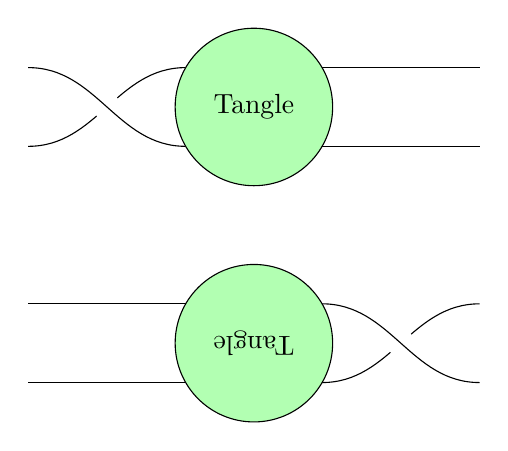
\begin{tikzpicture}
    \draw (0,0) to[out=0, in=180] (2, 1);
    \fill[white] (1, 0.5) circle (5pt);
    \draw (0,1) to[out=0, in=180] (2, 0);
    \filldraw[fill=green!30] ({2+sqrt(1-0.25)}, 0.5) circle (1);
    \draw ({2+2*sqrt(1-0.25)}, 1)--({4+2*sqrt(0.75)}, 1);
    \draw ({2+2*sqrt(1-0.25)}, 0)--({4+2*sqrt(0.75)}, 0);
    \node at ({2+sqrt(0.75)}, 0.5) {Tangle};

    \begin{scope}[shift={ ({4+2*sqrt(0.75)}, -2) }, rotate=180]
      \draw (0,0) to[out=0, in=180] (2, 1);
      \fill[white] (1, 0.5) circle (5pt);
      \draw (0,1) to[out=0, in=180] (2, 0);
      \filldraw[fill=green!30] ({2+sqrt(1-0.25)}, 0.5) circle (1);
      \draw ({2+2*sqrt(1-0.25)}, 1)--({4+2*sqrt(0.75)}, 1);
      \draw ({2+2*sqrt(1-0.25)}, 0)--({4+2*sqrt(0.75)}, 0);
      \node[rotate=180] at ({2+sqrt(0.75)}, 0.5) {Tangle};
    \end{scope}
  \end{tikzpicture}
  \caption{\label{flype}Wywracanie skarpety na lewą stronę, czyli \emph{flype}.}
\end{figure}

Słowo \emph{flype} pochodzi ze szkockiego i oznacza wywracanie skarpetki na lewą stronę. Chodzi o obracanie kołtuna (ang. \emph{tangle}) o 180 stopni (patrz. \cref{flype} lub \href{https://en.wikipedia.org/wiki/Flype}{wikipedia <3}). Kołtun to włożenie $n$ łuczków w $S^3$ tak, że ich $2n$ końców jest przyklejonych do $2n$ punktów zaznaczonych na granicy $S^3$.

Do pierwszego punktu twierdzenia wyżej powrócimy później. %Resztę zignorujemy.

\subsection{Linki rozszczepione (ang. \emph{split}) i pierwsze}

\begin{deff}[link i diagram rozszczepiony]
  Powiemy, że \buff{link $L$} (o co najmniej dwóch komponentach) zanurzony w $S^3$ jest \buff{rozszczepiony}, jeśli możemy $S^3$ podzielić na dwie kule $S^2$ tak, że każda ma po przynajmniej jednym komponencie $L$. 

  Definicja ta przenosi się na diagram $D\in S^2$ poprzez spłaszczenie tych sfer $S^2$ do zamkniętych krzywych. To znaczy, \buff{diagram $D$ jest rozszczepiony}, jeśli istnieje prosta krzywa zamknięta w $S^2\setminus D$, która dzieli je na dwa rozłączne dyski, każdy zawierający przynajmniej jeden komponent $D$.
\end{deff}

Link trywialny, czyli $O\;O$, jest w oczywisty sposób rozszczepialny. 

Link Whitehead'a (patrz \cref{whitehead link}) nie jest rozszczepialny. Aby to pokazać, wystraczy zauważyć, że link Whitehead'a składa się z dwóch trywialnych węzłó $O$. Gdyby więc był rozszczepialny, to moglibyśmy przekształcić \cref{whitehead link} w diagram $O\;O$, którego wielomian Jonesa wynosi $V(O\;O)=(-t^{\frac{1}{2}}-t^{-\frac{1}{2}})$. Wielomian Jonesa linku Whitehead'a wynosi natomiast $V(\text{Whitehead})=t^{-\frac{3}{2}}(-1+t-2t^2+t^3-2t^4+t^5)$. Ewidentnie coś się nie zgadza.

\begin{figure}[h]\centering 
  %\subfloat[][alternujący diagram]{
  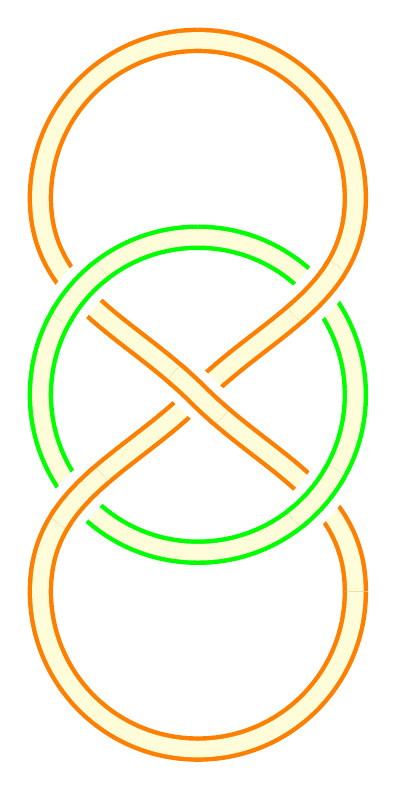
\begin{tikzpicture}
    \begin{knot}[
      clip width=20,
      %consider self intersections, 
      %draft mode=crossings,
      flip crossing=2,
      flip crossing=5,
      flip crossing=1,
      line join=round
      ]
      \strand[thick,
      background color=white,
        only when rendering/.style={
        draw=green,
        ultra thick,
        double=yellow!15,
        double distance=6pt,
        %line cap=round,
      }
      ] (90:2) to[out=0, in=90]
      (0:2) to[out=-90, in=0] 
      (-90:2) to[out=180, in=-90] 
      (180:2) to[out=90, in=180] 
      (90:2);
      \strand[thick,
      background color=white,
        only when rendering/.style={
        draw=orange,
        ultra thick,
        double=yellow!15,
        double distance=6pt,
        %line cap=round,
      }
      ] (90:2+2.5) to[out=0, in=90] 
      (2,2.5) to[out=-90, in=45]
      (0,0) to[out=180+45, in=90]
      (-2, -2.5) to[out=-90, in=180]  
      (0, -4.5) to[out=0, in=-90]
      (2, -2.5);
      \strand[thick,
      background color=white,
        only when rendering/.style={
        draw=orange,
        ultra thick,
        double=yellow!15,
        double distance=6pt,
        %line cap=round,
      }
      ] (2, -2.5) to[out=90, in=-45]
      (0,0) to[out=180-45, in=-90] 
      (-2, 2.5) to[out=90, in=180] (0, 4.5);
    \end{knot}
\end{tikzpicture}
  \caption{\label{whitehead link}Link Whiteead'a nie jest rozszczepialny, ale jest alternujący.}
\end{figure}

\begin{thm}
  Link $L$ o alternującym diagramie $D$ jest rozszczepialny $\iff$ $D$ jest rozszczepialnym diagramem.
\end{thm}

\begin{proof}
  W książce Pana Lickorisha p.t. \emph{An Introduction To Knot Theory}, str. 36. Są ciekawsze rzeczy do powiedzenia.
\end{proof}
% {\color{red}
% Dowód tego twierdzenia zostanie podany na koniec sekcji.
% }

Na pierwszych zajęciach dowiedzieliśmy się, że nietrywialny węzeł $K$ jest pierwszy (ang. \emph{prime}), jeśli nie jest sumą spójną dwóch nietrywialnych węzłów. Moglibyśmy powiedzieć, że każda kula $S^2\subseteq S^3\setminus K$ przecinająca węzeł $K$ w dwóch punktach dzieli $S^3$ na dwa fragmenty, z czego jeden posiada "trywialny łuczek", tj. łuczek który bez problemu możemy rozsupłać przy pomocy ruchów Reidenmeistera. W podobny sposób możemy przenieść definicję pierwszości na linki i ich diagramy.

\begin{deff}[link i diagram pierwszy]
  \buff{Link $L\subseteq S^3$}, różny od linku (i węzła) trywialnego, jest \buff{pierwszy}, jeśli każda sfera $S^2$ przecinająca go w dwóch punktach dzieli $S^3$ na dwa fragmenty, z których jeden zawiera jeden trywialny łuczek $L$.

  \buff{Diagram $D\subseteq S^2$ jest pierwszy}, jeśli każda prosta krzywa zamknięta w $S^2$ przecinająca $D$ w dwóch punktach zawiera w swoim wnętrzu lub na zewnątrz diagram odpowiadający rozwiązywalnemu łuczkowi. Takie $D$ jest \acc{silnie pierwszy}, jeśli zawsze po takim rozcięciu znajdziemy diagram z zerową liczbą skrzyżowań. 
\end{deff}

Tutaj warto zauważyć, że jedynym linkiem, który jest jednocześnie pierwszy i rozszczepiony jest link trywialny $O\;O$.

Kolejne twierdzenie, na którego dowód musimy troszkę poczekać, które pozwala nam badać pierwszość linków alternujących przez pryzmat ich diagramów.
\begin{thm}
  Załóżmy, że $L$ jest linkiem o alternującym diagramie $D$. Wtedy $L$ jest linkiem pierwszym $\iff$ $D$ jest diagramem pierwszym.
\end{thm}

%{\large\color{red}WRÓCIĆ TUTAJ, BO MI SIĘ CHWILOWO NIE CHCE}
\begin{proof}
  Tak jak i wcześniej, odsyłam do książki pana Lickorisha.
\end{proof}

\subsection{Po co nam to wszystko? Czyli o jeżach (między innymi)}

Zacznijmy od szybkiej informacji co to znaczy być powierzchnią. Oczywiście mówiąc powierzchnia mamy na myśli $2$-rozmaitość, czyli przestrzeń której każdy punkt ma otoczenie homeomorficzne z otwartym podzbiorem $\R^2$. Zamkniętych powierzchni nie ma bardzo dużo i każda taka powierzchnia jest wymieniona niżej
\begin{enumerate}
  \item sfera $S^2$
  \item suma spójna $n$ torusów $\mathbb{T}^2$
  \item suma spójna $n$ płaszczyzn rzutowych $\R P^2$
\end{enumerate}
Poza tym jest m.in. butelka Kleina (nieorientowalna, bez brzegu) czy wstęga M\"obiusa (nieorientowalna, z brzegiem).

Powiemy teraz, co to znaczy, że powierzchnia $F\subseteq M$, gdzie $M$ jest $3$-rozmaitością, jest niekompresowalna. Przy okazji dowiemy się, co to znaczy być dyskiem rozpinającym powierzchnię.

\begin{deff}[powierzchnia niekompresowalna] 
  Niech $F$ będzie powierzchnią różną od $S^2$ zanurzoną w $3$-rozmaitość $M$. Powiemy, że $F$ jest \buff{niekompresowalna}, jeśli każdy dysk $\Delta\subseteq M$ taki, że $\Delta\cap F=\partial\Delta$ (tzn. $\Delta$ \acc{rozpina} powierzchnię $F$) ogranicza dysk w $F$ (patrz \cref{pierwszy}).

  Sfera $S^2$ jest niekompresowalna, jeśli nie ogranicza $D^3$ w $M$.
\end{deff}

\begin{figure}%
\centering
\subfloat[][powierzchnia niekompresowalna]{ 
  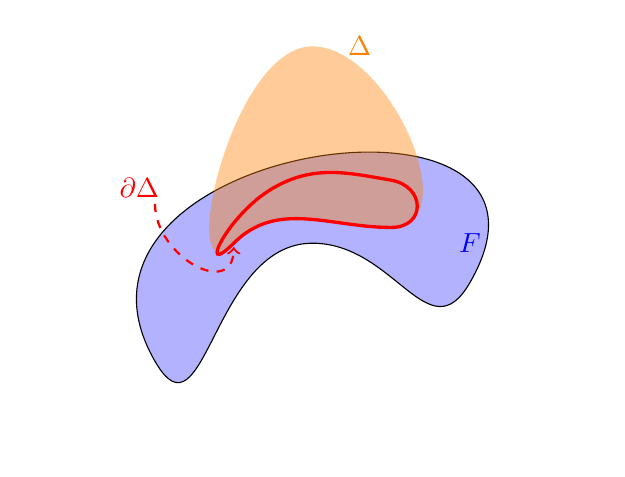
\begin{tikzpicture}
    \coordinate (a1) at (0,0);
    \coordinate (a2) at (-4, -1);
    \coordinate (a3) at (-2, 0.5);

    %\foreach \i in {1,...,3} \fill (a\i) circle (4pt);

    \filldraw[fill=blue!30] (a1) to[out=60, in=120, looseness=2] 
      (a2) to[out=-60, in=180, looseness=1.3] 
      (a3) to[out=0, in=-120, looseness=1.3] 
      (a1);
    \fill[opacity=0.4, orange] (-3, 0.5)to[out=45, in=180] (-1, 0.7) to[out=0, in=0] (-2, 3) to[out=180, in=180+45] (-3, 0.5);
    \draw[red, very thick] (-3, 0.5) to[out=45, in=180] (-1, 0.7) to[out=0, in=-10, looseness=1.9] (-1, 1.3) to[out=170, in=30, looseness=1] (-2.5, 1.2) to[out=210, in=180+45, looseness=2] (-3, 0.5);
    \draw[dashed, red, thick, ->] (-4, 1) to[out=-90, in=-90, looseness=1.5] (-3, 0.45);
    \node at (-4.2, 1.2) {$\color{red}\partial\Delta$};

    \node at (-1.4, 3) {$\color{orange}\Delta$};
    \node at (0, 0.5) {$\color{blue}F$};
  \end{tikzpicture}
}%
\qquad
\subfloat[][powierzchnia kompresowalna] {
  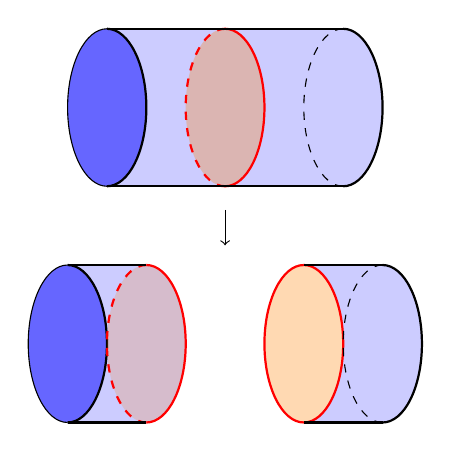
\begin{tikzpicture}
    \fill[blue!20] (0,0) rectangle (3, 2);
    \fill [blue!20] (3, 1) ellipse (0.5 and 1);
    \fill[blue!60] (0, 1) ellipse (0.5 and 1);

    \draw[thick] (0,0) arc (-90:90:0.5 and 1);
    \draw (0,0) arc (-90:-270:0.5 and 1);
    
    \fill[orange, opacity=0.3] (1.5, 1) ellipse (.5 and 1);
    \draw[thick, red] (1.5, 0) arc (-90:90:0.5 and 1);
    \draw[dashed, thick, red] (1.5,0) arc (-90:-270:0.5 and 1);
    
    \draw[thick] (3,0) arc (-90:90:0.5 and 1);
    \draw[dashed] (3,0) arc (-90:-270:0.5 and 1);
    \draw[thick] (0, 2)--(3, 2);
    \draw[thick] (0,0)--(3,0);

    \draw[->] (1.5, -0.3)--(1.5, -0.75);

    \begin{scope}[shift={(0, -3)}]
      \begin{scope}[shift={(-0.5, 0)}]
    \fill[blue!20] (0,0) rectangle (1, 2);
    \fill [blue!20] (1, 1) ellipse (0.5 and 1);
    \fill[blue!60] (0, 1) ellipse (0.5 and 1);

    \draw[thick] (0,0) arc (-90:90:0.5 and 1);
    \draw (0,0) arc (-90:-270:0.5 and 1);
    
    \fill[orange, opacity=0.2] (1, 1) ellipse (.5 and 1);
    \draw[thick, red] (1, 0) arc (-90:90:0.5 and 1);
    \draw[dashed, thick, red] (1,0) arc (-90:-270:0.5 and 1);
    
    % \draw[thick] (1,0) arc (-90:90:0.5 and 1);
    % \draw[dashed] (1,0) arc (-90:-270:0.5 and 1);
    \draw[thick] (0, 2)--(1, 2);
    \draw[thick] (0,0)--(1,0);
  \end{scope}


    \begin{scope}[shift={(0.5, 0)}]
    \fill[blue!20] (2,0) rectangle (3, 2);
    \fill [blue!20] (3, 1) ellipse (0.5 and 1);

    %\draw[thick] (0,0) arc (-90:90:0.5 and 1);
    %\draw (0,0) arc (-90:-270:0.5 and 1);
    
    \fill[orange!30] (2, 1) ellipse (.5 and 1);
    \draw[thick, red] (2, 0) arc (-90:90:0.5 and 1);
    \draw[thick, red] (2,0) arc (-90:-270:0.5 and 1);
    
    \draw[thick] (3,0) arc (-90:90:0.5 and 1);
    \draw[dashed] (3,0) arc (-90:-270:0.5 and 1);
    \draw[thick] (2, 2)--(3, 2);
    \draw[thick] (2,0)--(3,0);
  \end{scope}
  \end{scope}

  \end{tikzpicture}
}
\caption{\label{pierwszy} Powierzchnię (b) możemy rozciąć wzdłuż $\partial\Delta$ i zakleić dwoma kopiami $\Delta$, by dostać dwie "zakrętki" - powierzchnie o prostszej strukturze niż powierzchnia oryginalna. Jest tak, ponieważ otoczenie tubularne $\Delta$ ma ciekawy przekrój z $F$. W przypadku powierzchni (a) otoczenie tubularne $\Delta$ daje po prostu annulus na $F$. }%
\end{figure}

\begin{fuck}
  Niech $L$ będzie nierozszczepialnym, pierwszym i alternującym linkiem, a $F$ niech będzie zamkniętą niekompresowalną powierzchnią w $S^3\setminus L$. Wówczas istnieje dysk $\Delta$ rozpinający $F$ w $S^3$, który przecina $L$ w dokładnie jednym punkcie.
\end{fuck}

Żeby to zobaczyć, trzeba wyobrazić sobie \acc{najeżenie węzła/linku $L$}, czyli jego otoczenie tubularne (zamiast nitki mamy sznurek bawełniany o średnicy $5$mm). Takich otoczeń mamy dużo, dla każdego $\varepsilon>0$. Możemy więc wybierać otoczenia $U_n$ o średnicy $\frac{1}{n}$. Kiedy wyjmujemy z $S^3$ węzeł $K$ duża część $U_n$ zostaje, więc możemy wybierać duszczki $\Delta_n$, które mają przekrój z otoczneiem $U_n$ o średnicy $\frac{1}{n}$ na wysokości tylko jednego segmentu. Granica tych dyszczków nie jest już w $S^3\setminus L$, bo zahacza o otoczenie średnicy $0$, tzn. przecina się z węzłem $L$ w jednym punkcie.

\begin{fuck}
  Niech $L$ będzie nierozszczepialnym, pierwszym i alternującym linkiem. Każdy niekompresowalny torus $T$ zawarty w $S^3\setminus L$ jest równoległy do granicy najeżenia pewnego komponentu $L$.
\end{fuck}

Na przykład dla $L$ będącego linkiem o jednym elemencie, zawierającym tylko węzeł $3_1$, torusem równoległym do granicy jego najeżenia jest powierzchnia widoczna na \cref{najezenie trefoil}. Tak się składa, że link wyżej jest linkiem trywialnym, nierozszczepialnym i alternującym, więc tylko torus zawierające $L$ w swoim środku są niekompresowalne.

\begin{figure}[h]\centering
  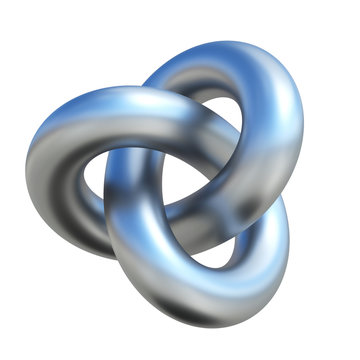
\includegraphics[width=0.5\textwidth]{trefoil-3d.jpg}
  \caption{\label{najezenie trefoil}Najeżenie węzła $3_1$.}
\end{figure}

Może nas to interesować, gdyż $3$-rozmaitości $M$, w których wszystkie niekompresowalne torusy są granicami najeżenia pewnego linku, zwykle posiadają strukturę hiperboliczną (pisał o tym pan W. P. Thurston i po przepisaniu do \LaTeX wyszło 379 stron pdf, który można znaleźć \href{https://www.math.unl.edu/~jkettinger2/thurston.pdf}{tutaj}). Hiperboliczność $3$-rozmaitości definiujemy przy pomocy metryki riemannowskiej i krzywizn, ale można to uprościć do stwierdzenia, że hiperboliczność oznacza brak materiału (sformułowanie ukradzione A. Karolakowi), czyli m.in. trójkąciki wtedy mają kąty sumujące się do mniej niż $\pi$.

\begin{deff}[sfera Conwaya]
  Dla linku $L\subseteq S^3$ $2$-sferę $\Sigma$ (tzn. $\Sigma=S^2$), która przecina $L$ w $4$ punktach nazywamy \buff{sferą Conwaya}, jeśli 
  \begin{enumerate}
    \item $\Sigma\setminus L$ jest niekompresowalne w $S^3\setminus L$
    \item każde $S^2\subseteq S^3\setminus \Sigma$ przecinające $L$ w dwóch punktach odcina niezawiązany segment $L$. 
  \end{enumerate}
\end{deff}

Tutaj moglibyśmy temat drążyć dalej, ale niestety pojawia się następujący fragment tekstu w Lickorishu

\begin{adjustwidth}{5cm}{5cm}
\begin{center}
  \slshape 
  They \emph{[Bonahon and Siebenmann]} show that for any knot that is not a
satellite, there is a well-defined maximal collection of Conway spheres that divides
the knot into an arborescent part and a part in which any Conway sphere is pairwise
parallel to a boundary component.
\end{center}
\end{adjustwidth}

po przeczytaniu którego autor tej notatki postanowił ograniczyć się do wklejenia przykładu sfery Conwaya w \cref{conway sphere}, zaczerpniętego z \href{https://en.wikipedia.org/wiki/Conway_sphere#/media/File:Algebraic_Borromean_link_diagram.svg}{wikipedii}
\begin{figure}[h]\centering
  
\includegraphics[width=0.7\textwidth]{conway-sphere.png}
  \caption{\label{conway sphere}Przerywana linia to sfera Conwaya dla $L=$pierścienie boromejskie.}
\end{figure}

\subsection{Stany diagramu}

Tydzień temu przypisywaliśmy skrzyżowaniom wartość $\pm1$. Dzisiaj nazwiemy taką właśnie funkcję $s:[n]\to \{1, -1\}$, gdzie $n$ to ilość skrzyżowań badanego diagramu linku $D$.

\begin{deff}
  Niech $D$ będzie diagramem linku $L$ o $n$ skrzyżowaniach. Funkcję $s:\{1,..., n\}\to \{1, -1\}$ nazywamy \buff{stanem} diagramu $D$.
\end{deff}

Stanów jest $2^n$, ale spośród nich wyróżniają się dwa konkretne: $\color{blue}s_+$ i $\color{blue}s_-$, przypisujące odpowiednio $1$ i $-1$ wszystkim skrzyżowaniom.

Mając dany stan $s$ i diagram $D$ możemy określić nowy diagram $sD$, który przypisuje $i$-temu skrzyżowaniu odpowiednie jego odkrzyżowanie, w zależności od wartości $s(i)$ w sposób zdefiniowany na \cref{stan od diagramu}. 

\begin{figure}[h]\centering 
  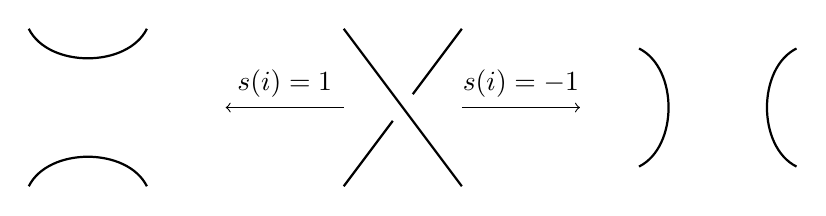
\begin{tikzpicture}
    \begin{scope}[shift={(-1, 0)}]
      \draw[thick] (0,0)..controls (0.25, -0.5) and (1.25, -0.5)..(1.5, 0);
      \draw[thick] (0,-2)..controls (0.25, -1.5) and (1.25, -1.5)..(1.5, -2);
    \end{scope}

    \draw[thick] (3, -2)--(4.5, 0);
    \fill[white] (3.75, -1) circle (6pt);
    
    \draw[thick] (3, 0)--(4.5, -2);
    \begin{scope}[shift={(7, 0)}, rotate around={90:(0.75, -1)}]
      \draw[thick] (0,0)..controls (0.25, -0.5) and (1.25, -0.5)..(1.5, 0);
      \draw[thick] (0,-2)..controls (0.25, -1.5) and (1.25, -1.5)..(1.5, -2);
    \end{scope}

    \draw[->] (3, -1)-- node[midway, above] {$s(i)=1$} (1.5, -1);
    \draw[->] (4.5, -1)-- node[midway, above] {$s(i)=-1$} (6, -1);
  \end{tikzpicture}
  \caption{\label{stan od diagramu}Zasada zamiany skrzyżowań w $sD$.}
\end{figure}
Wynikowy diagram $sD$ nie posiada skrzyżowań (wszystkie wycięliśmy), ale posiada $|sD|$ zamkniętych krzywych. 

Teraz możemy zdefiniować, w dość bolesny sposób, \buff{nawias Kauffmanna} przy pomocy stanów diagramu $D$:
$$\langle D\rangle = \sum_s\left[A^{\sum_{i\geq 1} s(i)}(-A^{-2}-A^2)^{|sD|-1}\right].\quad \quad (\star)$$
Zauważmy, że jest to dokładnie to samo, co pisaliśmy tydzień temu, z tym że tym razem nie wykorzystujemy rekurencji.

\begin{fuck}
  Wzór $(\star)$ jest naprawdę nawiasem Kauffmanna sprzed tygodnia.
\end{fuck}


\def\iksik{\tikz[baseline=.1ex]{
  \draw[thick] (0,0)--(1.5ex, 1.5ex);
  \fill[white] (0.75ex, 0.75ex) circle (2pt);
  \draw[thick] (0,1.5ex)--(1.5ex, 0);
  }
}

\def\lewoprawo{\tikz[baseline=.1ex]{
    \draw[thick] (0,0)..controls(.5ex, .25ex)and(.5ex, 1.25ex)..(0,1.5ex);
    \draw[thick] (1.5ex,0)..controls(1ex, .25ex)and(1ex, 1.25ex)..(1.5ex,1.5ex);
  }
}

\def\goradol{\tikz[baseline=.1ex]{
    \draw[thick] (0,0)..controls(.25ex, .5ex)and(1.25ex, .5ex)..(1.5ex,0);
    \draw[thick] (0,1.5ex)..controls(.25ex, 1ex)and(1.25ex, 1ex)..(1.5ex,1.5ex);
  }
}

\begin{proof}
  Oznaczając wartość $(\star)$ przez $[D]$ mamy do pokazania $3$ kroki
  \begin{enumerate}
    \item $[O]=1$
    \item $[D\sqcup O]=(-A^{-2}-A^2)[D]$
    \item $[\iksik]=A[\lewoprawo]+A^{-1}[\goradol]$
  \end{enumerate}

  (1) wychodzi od razu z faktu, że $O$ ma dokładnie jeden stan pusty, czyli $\sum_{i\geq 1}s(i)=0$ i $|sO|=1$. Równość numer (2) wynika z faktu, że $D\sqcup O$ na $D$ zachowuje się dokładnie tak samo jak $D$, ale z racji $O$ dochodzi jedna krzywa zamknięta. Stąd 
  $$[D\sqcup O]=\sum_s\left[A^{\sum_{i\geq 1}s(i)}(-A^{-2}-A^2)^{|sD|+1-1}\right=\sum_s\eft[A^{\sum_{i\geq 1}s(i)}(-A^{-2}-A^2)^{|sD|-1}\right](-A^{-2}-A^2).$$

  Ostatnia równość wynika z faktu, że diagramy $\goradol$ i $\lewoprawo$ nie mają stanów różnych od $s_+$ i $s_-$ diagramu $\iksik$
  \begin{align*}
    A[\lewoprawo]&=A(-A^{-2}-A^2)^{2-1}A\\ 
                 &=A(-A^{-2}-A^2)^{|\iksik|-1}A^{s_-(x)-1}=\\ 
                 &=(-A^{-2}-A^2)^{|\iskik|-1}A^{s_-(x)}\\
    A^{-1}[\goradol]&=A^{-1}(-A^{-2}-A^2)^{2-1}A^{-1}=\\ 
                    &=A^{-1}(-A^{-2}-A^2)^{|\iksik|-1}A^{s_+(x)+1}\\
                 &=(-A^{-2}-A^2)^{|\iskik|-1}A^{s_+(x)}
  \end{align*}
  gdzie $x$ to jedyne skrzyżowanie w $\iksik$. Po dodaniu wszystko się zgadza.
\end{proof}

Wprowadźmy teraz kolejne pojęcie dotyczące diagramów, tj. ich fajności (po angielsku nazywamy to \emph{adequate}, ale wydaje mi się to dojść niemiłym określeniem diagramów, które naprawdę się starają).

\begin{deff}[diagram fajny]
  Powiemy, że diagram $D$ jest \buff{fajny}, jeśli dla wszystkich stanów $s$ takich, że $\sum_{i\geq 1}s(i)=n-2$ zachodzi $|s_-D|>|sD|$ i $|s_+D|>|sD|$. Jeśli tylko jedna nierówność to jest on odpowiednio $-$ lub $+$ fajny.
\end{deff}

Po co nam to wszystko? Okazuje się, że najmniejsze diagramy alternujące są zawsze fajne c:

\begin{fuck}
  Zredukowany diagram alternujący $D$ jest zawsze fajny.
\end{fuck}

\begin{proof}
  Pomalujmy wnętrze diagramu na niebiesko i pomarańczowo naprzemiennie, jak np. widać na \cref{szachownica diagramowa} (a). Ponieważ węzeł jest alternujący, to wiemy, że $s_+D$ zachowa tylko fragmenty pomalowane na jeden kolor, np. czerwony jak na rysunku niżej. Z kolei $s_-D$ otrzyma tylko połacie niebieskie. Dzięki brakowi zbędnych krawędzi nie będziemy mieli dwóch fragmentów, które zleją się w jedność, jak np. na \cref{szachownica diagramowa} (b) po rozcięciu zaznaczonym na czerwono. 

  Zamieniając dwa skrzyżowania na przeciwną wartość $s$ połączymy dwa lub więcej fragmenty różnego koloru w jeden, więc dostaniemy ich zawsze mniej niż w przypadku gdy wszystkie skrzyżowania miały tę samą wartość $s$.

  \begin{figure}[h]\centering
    \subfloat[][diagram bez zbytku]{
    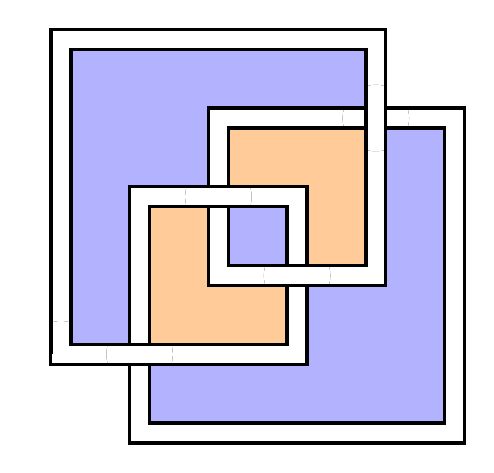
\begin{tikzpicture}
      \filldraw[fill=blue!30] (0, -4)--(0,0)--(4, 0)--(4, -1)--(2, -1)--(2, -2)--(1, -2)--(1, -4)--(0, -4);
      \filldraw[fill=orange!40] (4, -1)--(2, -1)--(2, -2)--(3, -2)--(3, -3)--(4, -3)--(4, -1);
      \filldraw[fill=orange!40] (1, -4)--(3, -4)--(3, -3)--(2, -3)--(2, -2)--(1, -2)--(1, -4);
      \filldraw[fill=blue!30] (2, -3)--(3, -3)--(3, -2)--(2, -2)--(2, -3);
      \filldraw[fill=blue!30] (1, -4)--(1, -5)--(5, -5)--(5, -1)--(4, -1)--(4, -3)--(3, -3)--(3, -3)--(3, -4)--(1, -4);
      \begin{knot}[ 
        consider self intersections,
        ignore endpoint intersections=false,
        clip width=2,
        %draft mode=crossings,
        background color=white,
        only when rendering/.style={
          draw=black,
          double=white,
          double distance=6pt, 
          %line cap=round
        },
        flip crossing=2,
        flip crossing=5,
        flip crossing=6
        ]
        \strand[very thick] 
          (0, -4) to 
          (0, 0) to 
          (4, 0) to 
          (4, -3) to 
          (2, -3) to 
          (2, -1) to 
          (4, -1) to 
          (5, -1) to 
          (5, -5) to 
          (1, -5) to 
          (1, -2) to 
          (3, -2) to 
          (3, -4) to 
          (0, -4);
      \end{knot}
      \fill[white] (-0.1, -4.09) rectangle (0.18, -3.9);
      \draw[very thick](-0.13, -4)--(-0.13, -4.13)--(0.1, -4.13);


    \end{tikzpicture}
  }
  \subfloat[][diagram ze zbytkiem]{
    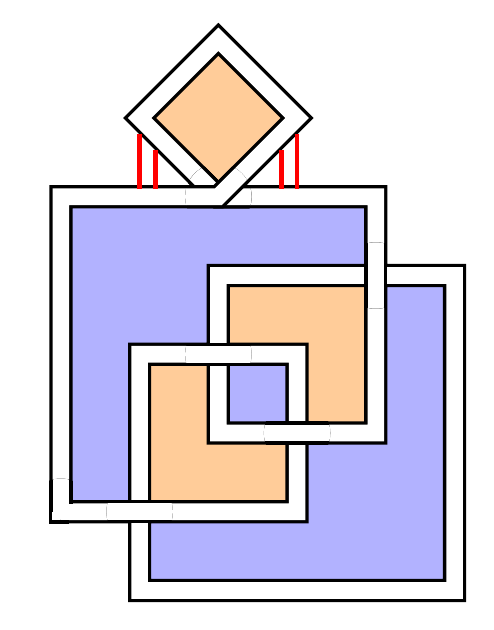
\begin{tikzpicture}
      \filldraw[fill=orange!40] (2, 0)--(3, 1)--(2,2)--(1,1)--(2,0);
      \filldraw[fill=blue!30] (0, -4)--(0,0)--(4, 0)--(4, -1)--(2, -1)--(2, -2)--(1, -2)--(1, -4)--(0, -4);
      \filldraw[fill=orange!40] (4, -1)--(2, -1)--(2, -2)--(3, -2)--(3, -3)--(4, -3)--(4, -1);
      \filldraw[fill=orange!40] (1, -4)--(3, -4)--(3, -3)--(2, -3)--(2, -2)--(1, -2)--(1, -4);
      \filldraw[fill=blue!30] (2, -3)--(3, -3)--(3, -2)--(2, -2)--(2, -3);
      \filldraw[fill=blue!30] (1, -4)--(1, -5)--(5, -5)--(5, -1)--(4, -1)--(4, -3)--(3, -3)--(3, -3)--(3, -4)--(1, -4);
      \begin{knot}[ 
        consider self intersections,
        ignore endpoint intersections=false,
        clip width=2,
        %draft mode=crossings,
        background color=white,
        only when rendering/.style={
          draw=black,
          double=white,
          double distance=6pt, 
          %line cap=round
        },
        flip crossing=2,
        flip crossing=8,
        flip crossing=9,
        flip crossing=3
        ]
        \strand[very thick] 
          (0, -4) to 
          (0, 0) to
          (2, 0) to (3, 1) to (2, 2) to (1, 1) to (2, 0) to
          (4, 0) to 
          (4, -3) to 
          (2, -3) to 
          (2, -1) to 
          (4, -1) to 
          (5, -1) to 
          (5, -5) to 
          (1, -5) to 
          (1, -2) to 
          (3, -2) to 
          (3, -4) to 
          (0, -4);
      \end{knot}
      \draw[ultra thick, red] (1, 0.8)--(1, 0.1);
      \draw[ultra thick, red] (3, 0.8)--(3, 0.1);
      \draw[ultra thick, red] (1.2, 0.6)--(1.2, 0.1);
      \draw[ultra thick, red] (2.8, 0.6)--(2.8, 0.1);

      \fill[white] (-0.1, -4.09) rectangle (0.18, -3.9);
      \draw[very thick](-0.13, -4)--(-0.13, -4.13)--(0.1, -4.13);

    \end{tikzpicture}
  }
    \caption{\label{szachownica diagramowa}Pomalowany diagram (węzła $4_1$).}
  \end{figure}
\end{proof}

\begin{fuck}
  Niech $D$ będzie nierozszczepionym diagramem o $n$ skrzyżowaniach. Wówczas
  $$|s_+D|+|s_-D|\leq n+2,$$
  z równością jeśli $D$ jest zredukowanym diagramem alternującym.
\end{fuck}

\begin{proof}
  Indukcja po ilości skrzyżowań $n$. Oczywiście dla $n=0$ mamy $LHS=0\leq 2=RHS$.

  Bierzemy teraz diagram $D$ o $(n+1)$ skrzyżowaniach i wybieramy jedno skrzyżowanie. Możemy je usunąć na dwa sposoby - sposób $+1$ lub $-1$, by powstał nowy diagram $D'$ o $n$ skrzyżowaniach. W którymś z tych przypadków dorysujemy nowy łuczek lub jakieś dwa łuczki nam się złączą w jedno. Drugi sposób zachowuje ilość łuczków. W takim razie z założenia indukcyjnego mamy
  $$|s_+D|+|s_-D|=|s_+D'|+|s_-D'|\pm 1\leq (n+2)\pm 1\leq n+3.$$
  W zredukowanym diagramie alternującym wystarczy zauważyć, że wycięcie skrzyżowania łączy dwa fragmenty jednego koloru.
\end{proof}

\subsection{W końcu wielomiany!}

Zaczniemy od zdefiniowania dwóch wartości zależnych od linku diagramu $D$ $L$: $M\langle D\rangle$ oraz $m\langle D\rangle$. Pierwsza z nich to maksymalna potęga wielomianu Jonesa, a druga - potęga minimalna. Oczywiście, jeśli węzeł jest swoim odbiciem lustrzanym, to $M\langle D\rangle = -m\langle D\rangle$.

Okazuje się, że wartości wyżej mają swoje odniesienie na stany węzła:
\begin{fuck}
  Niech $D$ będzie diagramem o $n$ skrzyżowaniach. Wówczas
  \begin{enumerate}
    \item $M\langle D\rangle \leq n+2|s_+D|-2$
    \item $m\langle D\rangle \geq -n-2|s_-D|+2$
  \end{enumerate}
  z równością gdy $D$ jest alternującym, zredukowanym diagramem.
\end{fuck}

\begin{proof}
  Dla dowolnego stanu $s$ oznaczmy $\langle D|s\rangle=(-A^{-2}-A^2)^{|sD|-1}A^{\sum s(i)}$. Wtedy mamy 
  $$\langle D\rangle = \sum_s \langle D|s\rangle$$
  Mamy $M\langle D|s\rangle=2|sD|-2+\sum s(i)$, w szczególności dla $s=s_+$ mamy interesującą nas wartość. Wystarczy pokazać, że dla każdego innego stanu $s$ mamy $\langle D|s\rangle \leq \langle D|s_+\rangle$.

  Weźmy więc dowolny stan $s\neq s_+$. Ma on $k$ znaków $-1$, możemy więc znaleźć ciąg $s_0=s,...,s_k=s_+$, gdzie w każdym kroku zmieniamy jeden $+1$ na $-1$. Oczywiście, dla każdego $j$ mamy 
  $$\sum s_{j+1}(i)=\sum s_j(i)+2,$$
  gdyż po zmianie $+1$ na $-1$ tracimy zerują nam się dwa $+1$.

  Z kolei $|s_{j+1}D|\pm 1=|s_jD|$ na podobnej zasadzie jak już wcześniej obserwowaliśmy. Z tego powodu 
  $$M\langle D|s_{j+1}\rangle =2|s_{j+1}D|-2+\sum s_{j+1}(i)=2|s_jD|\pm 2-2+\sum s_j(i)+2\geq 2|s_jD|-2+\sum s_j(i)=\langle D|s_j\rangle.$$

  Równość oczywiście zajdzie, jeśli nie będziemy w stanie nigdy mieć dwóch wyrazów z $M\langle D|s_+\rangle$ z przeciwnym znakiem w sumie, tzn. kiedy dla wszystkich stanów $s\neq s_+$ mamy $\langle D|s\rangle < \langle D|s_+\rangle$. Wystarczy tutaj zauważyć, że jeśli zmienimy wartość jednego skrzyżowania, to zlejemy w całość dwa fragmenty niebieskie na \cref{szachownica diagramowa}.

  Argument dla drugiej nierówności jest symetryczny.
\end{proof}

TO DO: span, pierwsze zdanie hipotez Taita.

\end{document}
